\documentclass[runningheads]{llncs}
\usepackage[text={150mm,220mm},centering]{geometry}
\usepackage{graphicx}
\usepackage{tikz}
\usepackage{float}
\begin{document}
\title{\large{CSCI814 IT Project Management (Lab2)}}
%--------------------Please do NOT change the content above.-------------------------------------------------

%
%----Please write your personal information as below.------------------------------------
%
\author{\large{Student Name: Wangzhihui Mei \\ % Please write your name here
        CCNU Student Number: 2019124044 \\ % Please write your CCNU student number here
        UOW Student Number: 6603385}}  % Please write your UOW student number here


%-----------------------------------------------------------------------------------------------



%---------Do not change the content of this part--------------------

\authorrunning{CCNU Wollongong Joint Institute}
\institute{Central China Normal University Wollongong Joint Institute}

\maketitle
\clearpage

%-----------Please write your solutions to the questions in the assignment from here.---------------

\section{In-class exercise}
\subsection{plan's costs per task}
\begin{figure}[H]
    \centering
    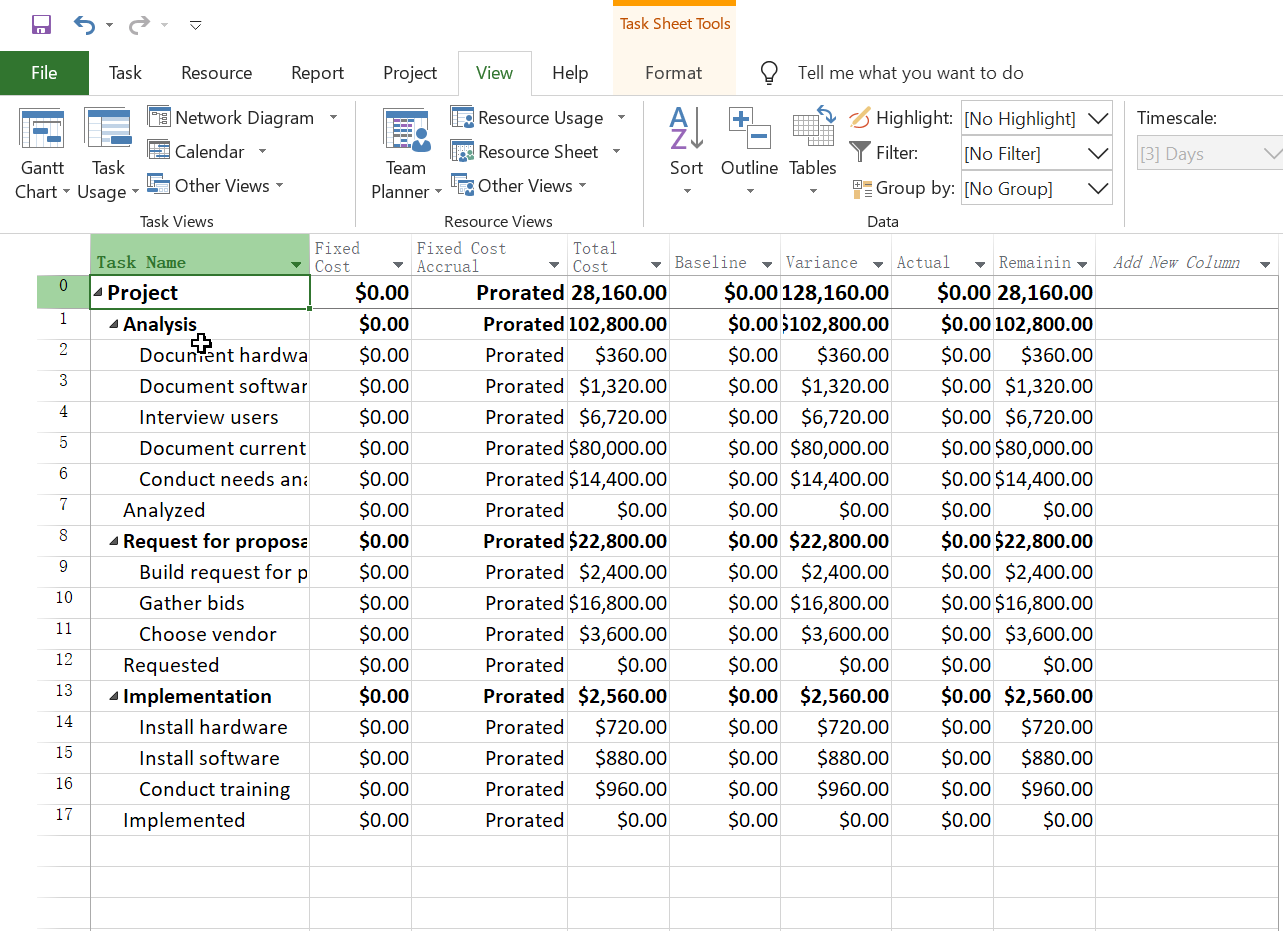
\includegraphics[width=1.0\textwidth]{./image/figure1}
    \caption{plan's costs per task}
    \label{}
\end{figure}

\subsection{plan's costs per resource}
\begin{figure}[H]
    \centering
    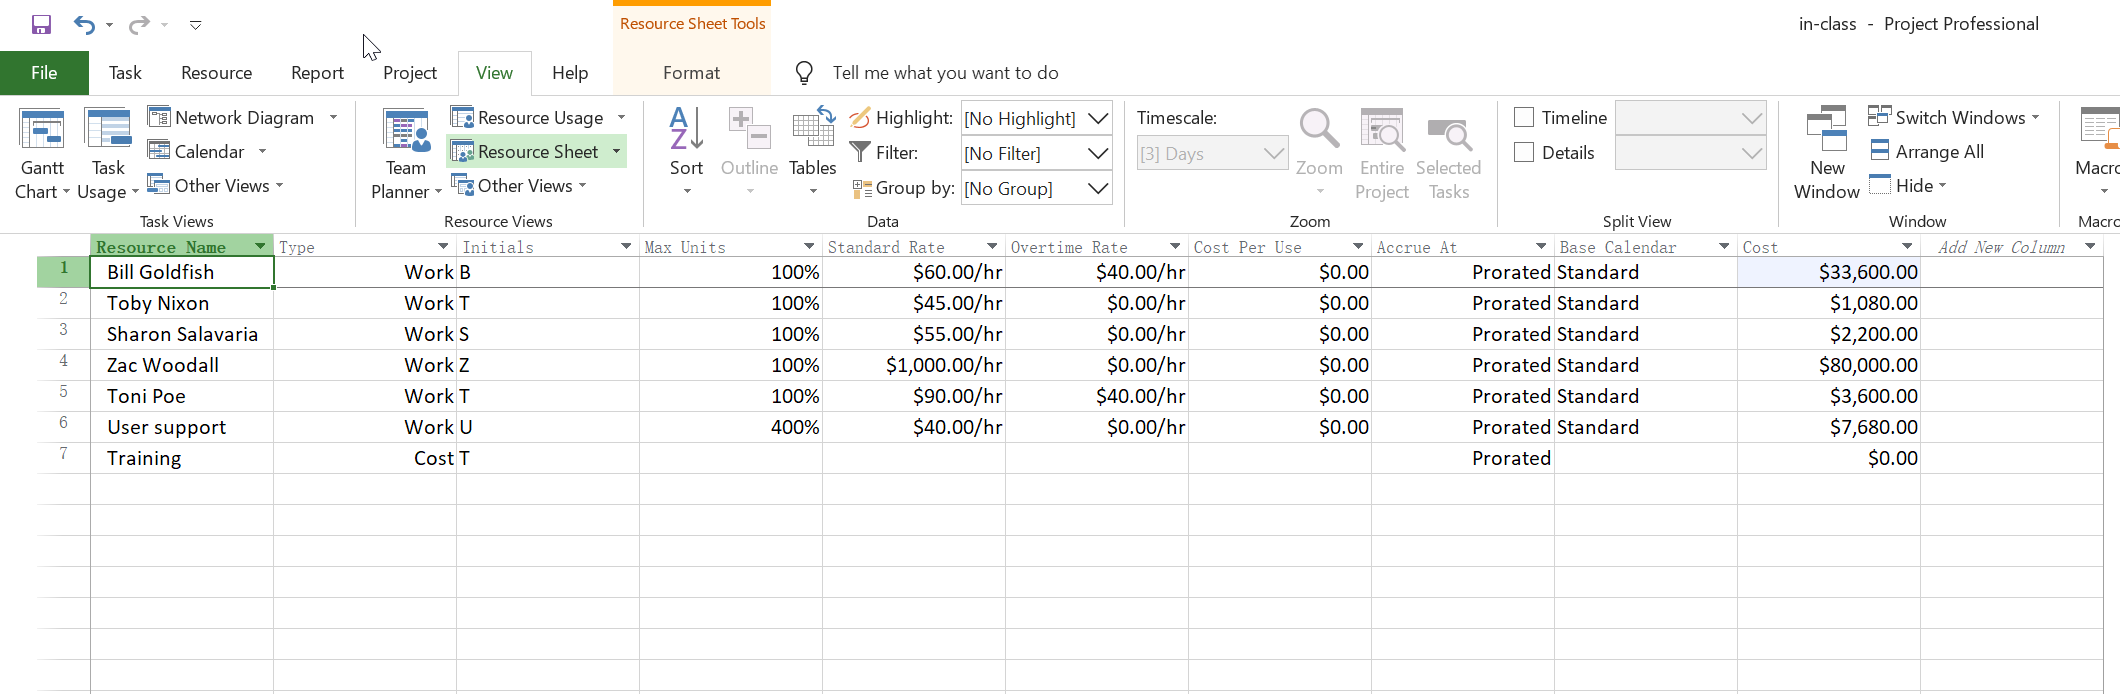
\includegraphics[width=1.0\textwidth]{./image/figure2}
    \caption{plan's costs per resource}
    \label{}
\end{figure}

\subsection{resource assignment grouped by task}
\begin{figure}[H]
    \centering
    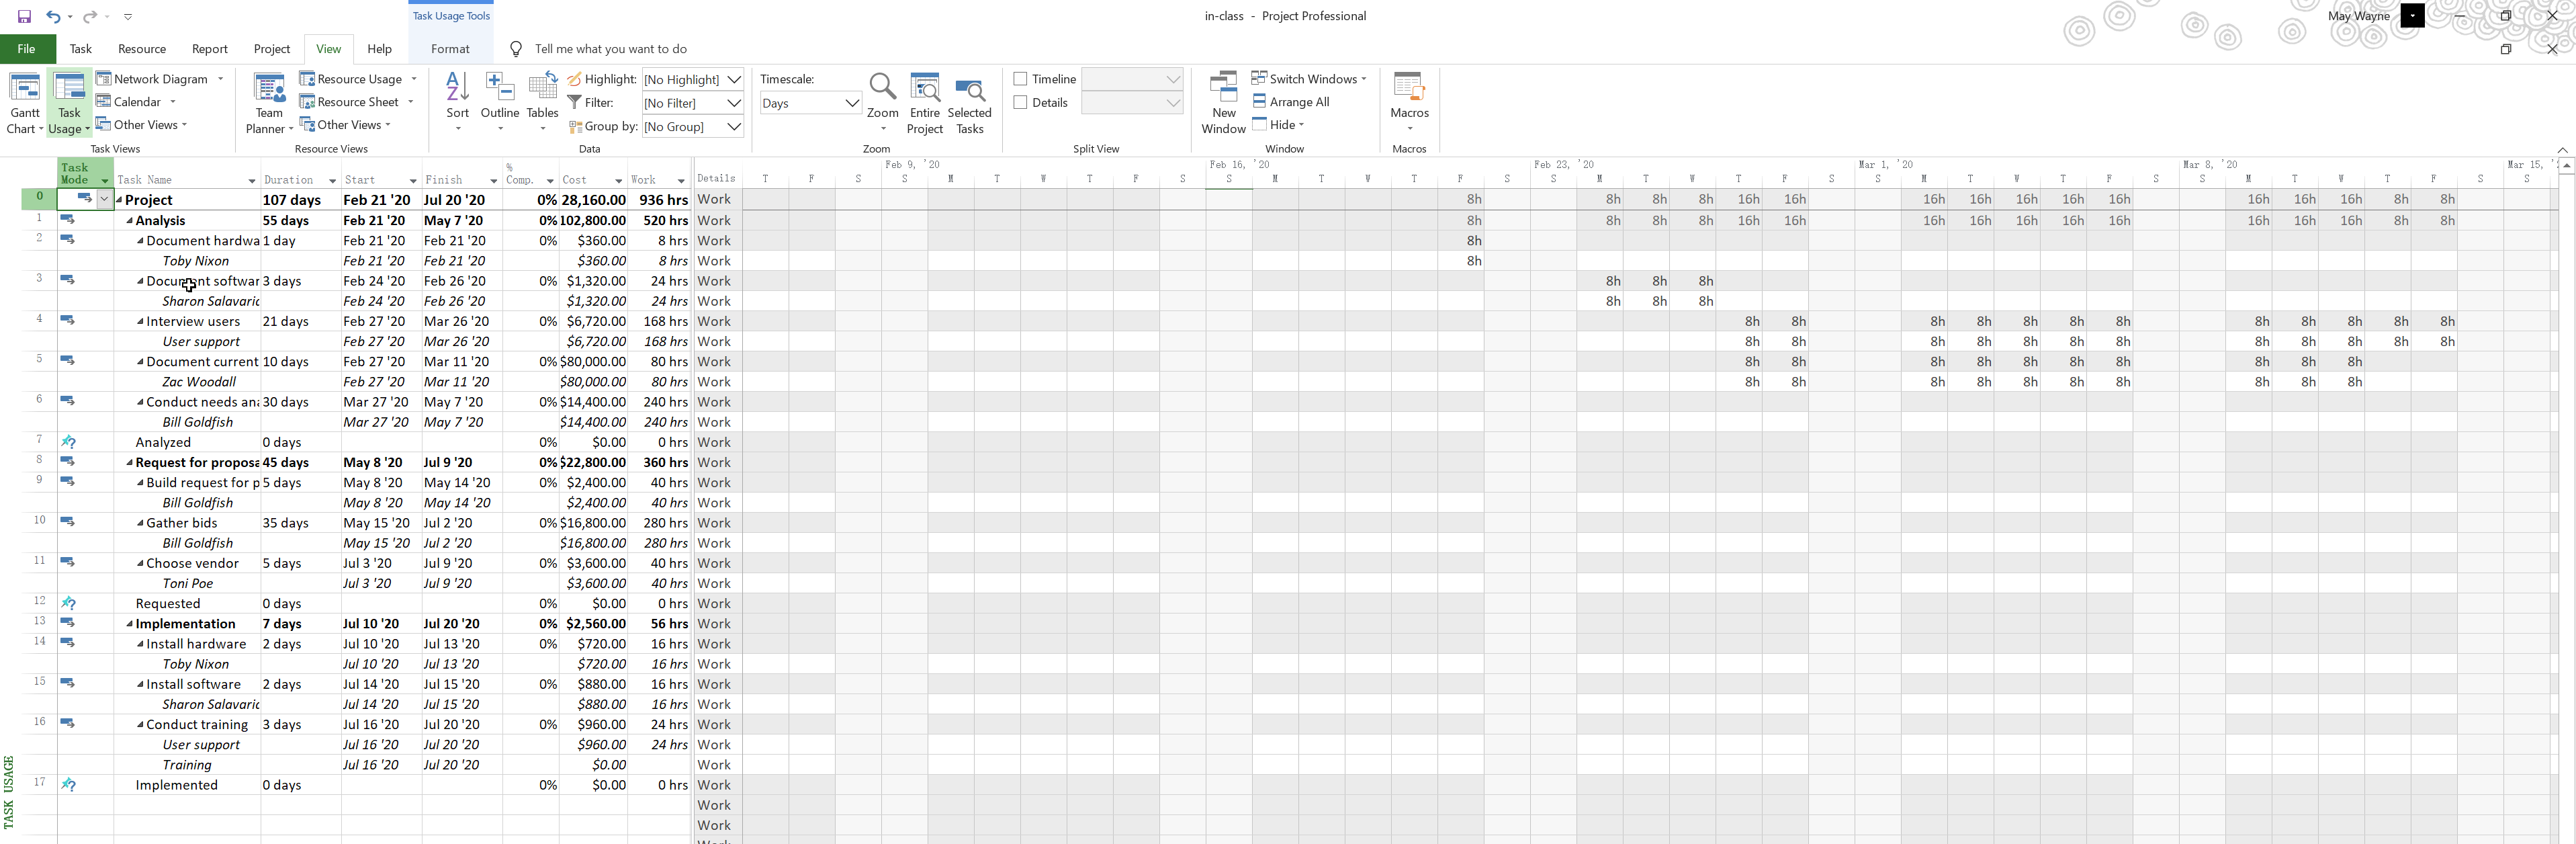
\includegraphics[width=1.0\textwidth]{./image/figure3}
    \caption{resource group by task}
    \label{}
\end{figure}

\subsection{task assignment grouped by resource}
\begin{figure}[H]
    \centering
    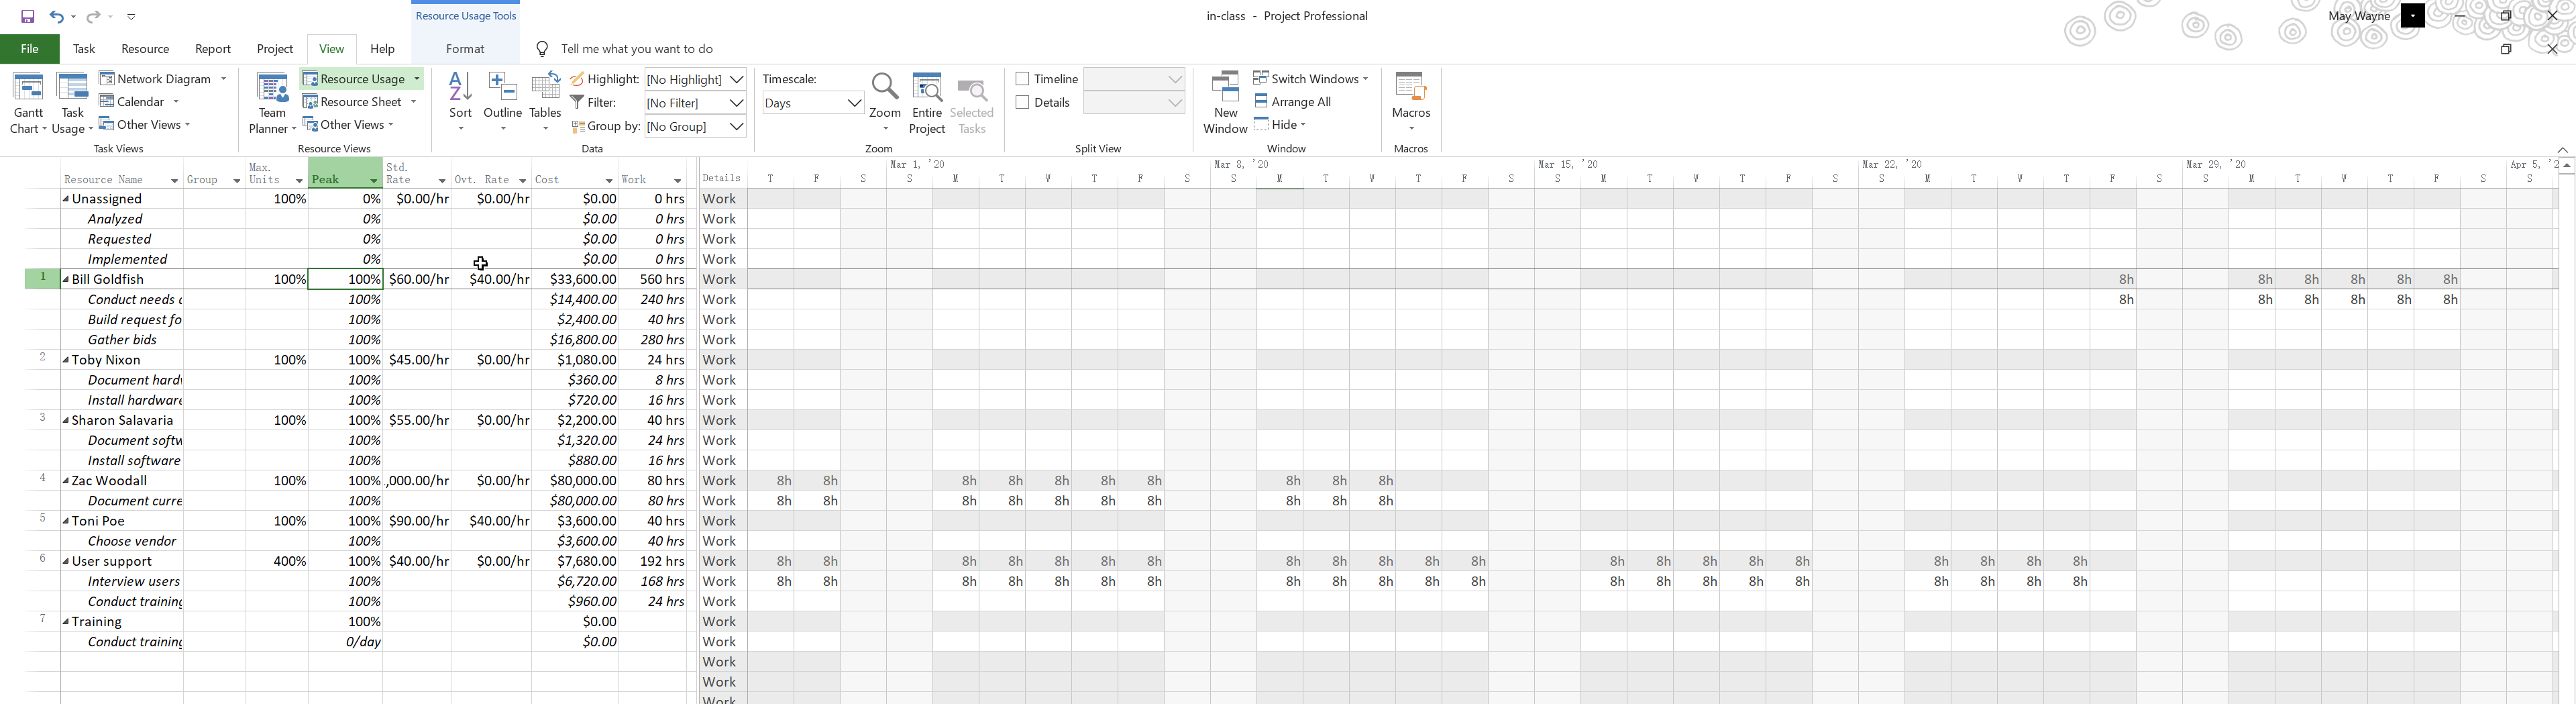
\includegraphics[width=1.0\textwidth]{./image/figure4}
    \caption{resource group by resource}
    \label{}
\end{figure}

\subsection{Others}

total cost is \$128160

\noindent
If Toby Nixon work part-time, the duration will change from 110 to 112 days while cost won't change.

\noindent
If Bill Goldfish don't work each Tuesday, the duration will change from 110 to 128 days while cost won't change.

\noindent
If adding Toni Poe as extra resource while keeping sam amount of work, the duration won't change while the project cost will fall to \$92120. If the duration remain constant, the project duration won't change while the cost will jump to \$135720.


\section{Lab1}
\subsection{Resource sheet}
\begin{figure}[H]
    \centering
    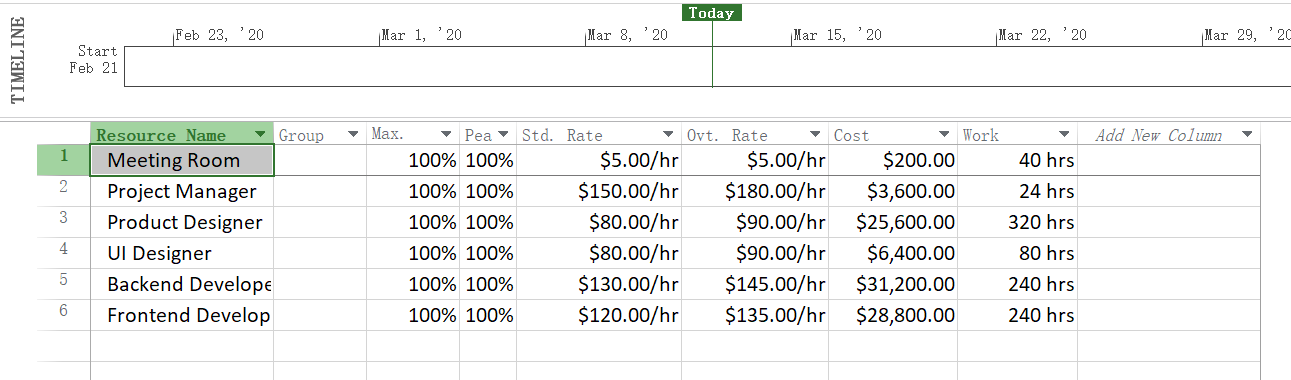
\includegraphics[width=1.0\textwidth]{./image/figure6}
    \caption{Resource sheet}
    \label{}
\end{figure}

\subsection{Task sheet}
\begin{figure}[H]
    \centering
    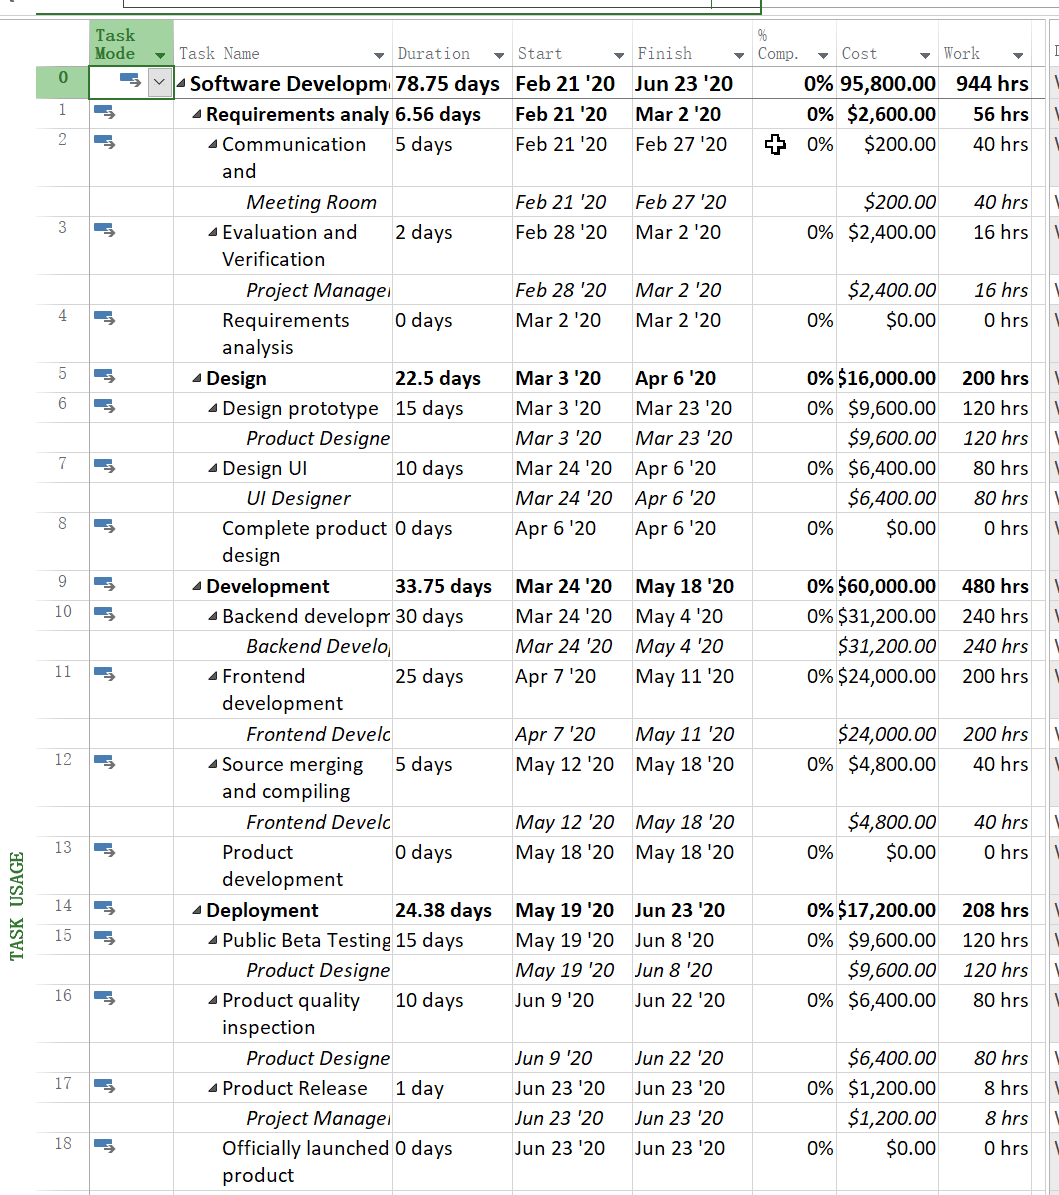
\includegraphics[width=1.0\textwidth]{./image/figure7}
    \caption{Task sheet}
    \label{}
\end{figure}

\subsection{Change of resource details}
\subsubsection{calendar/Working hours changing }
\subsection{Task sheet}
\begin{figure}[H]
    \centering
    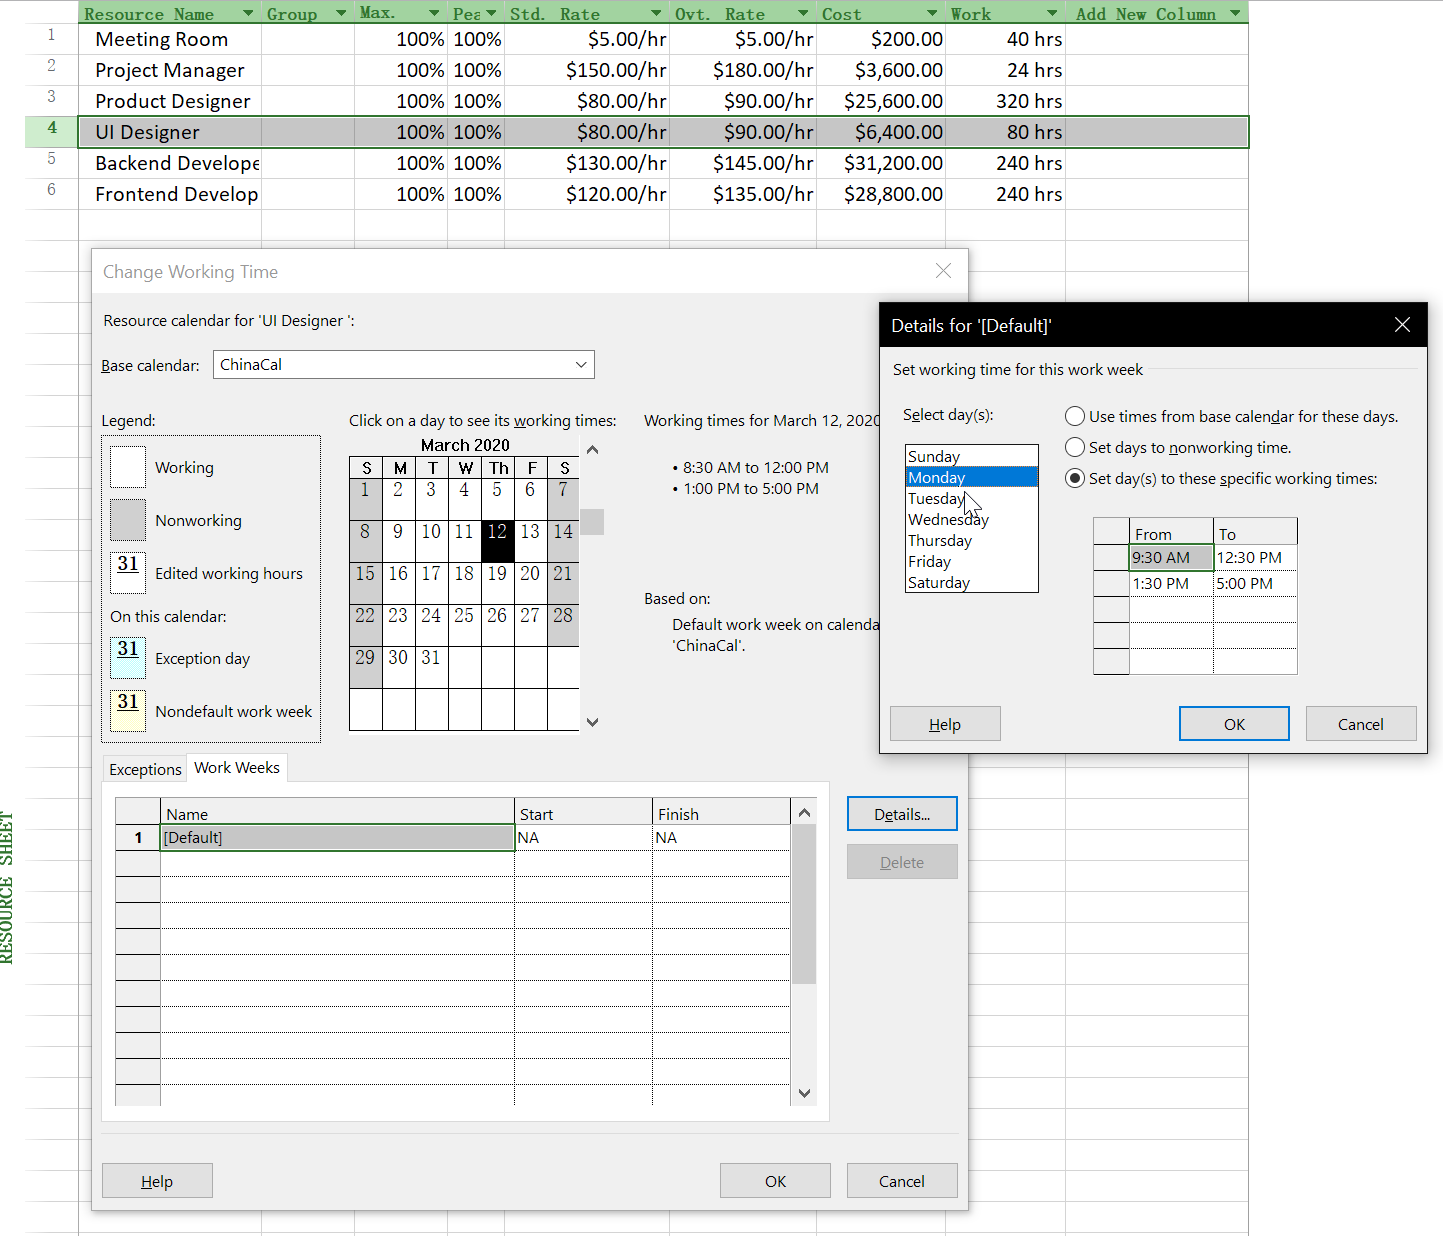
\includegraphics[width=1.0\textwidth]{./image/figure8}
    \caption{Resource details}
    \label{}
\end{figure}
Change calendar to Chinese public holiday calendar.
Change working hours from (Monday-Friday 8:30-17:00) to (Monday 9:30-17:00 Tuesday)

\subsection{Plan checking}
\begin{figure}[H]
    \centering
    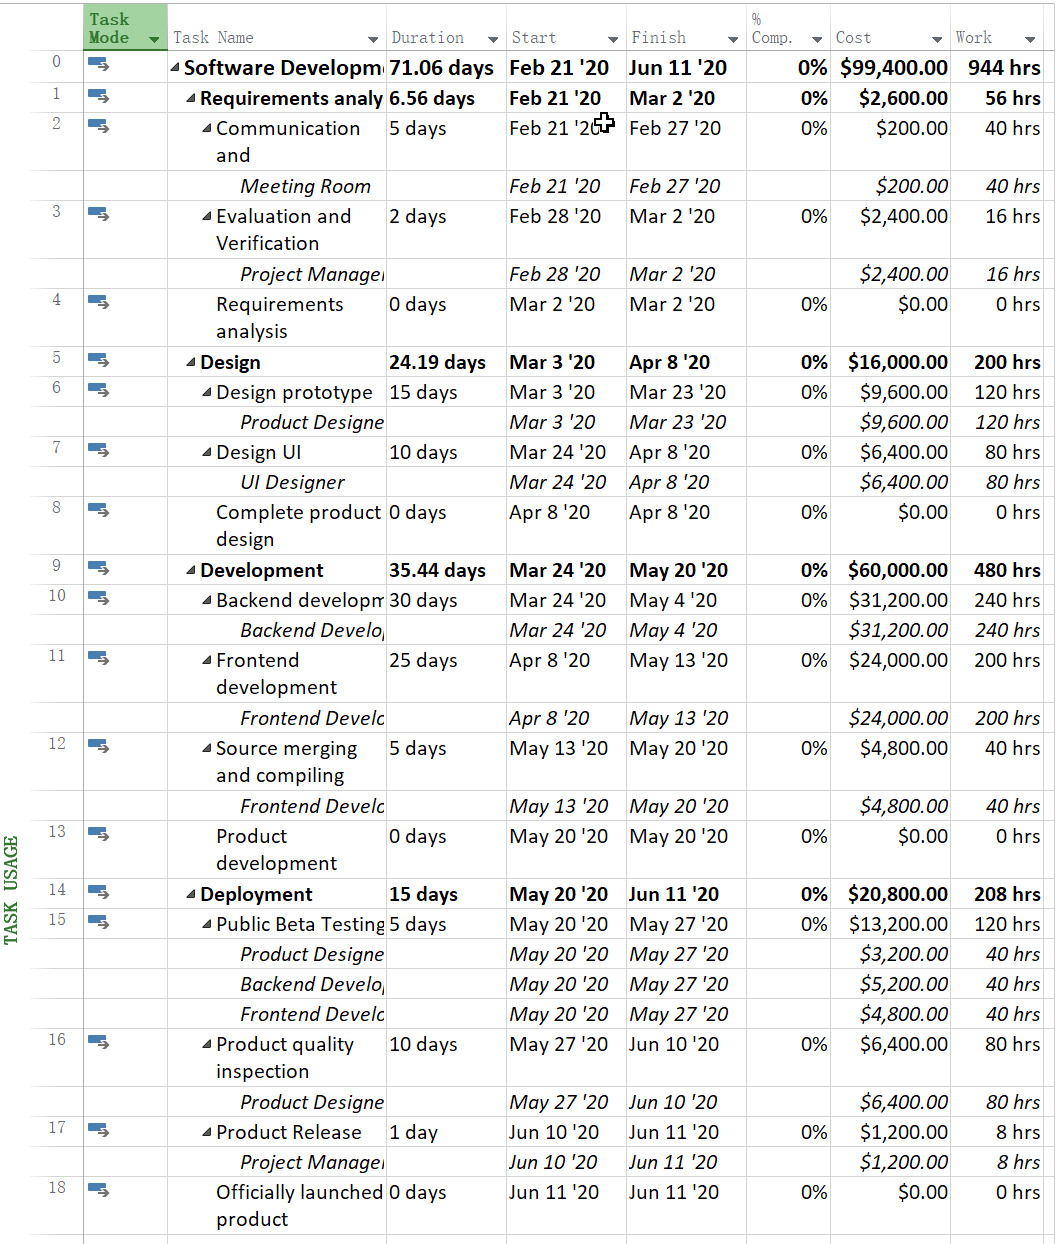
\includegraphics[width=1.0\textwidth]{./image/figure9}
    \caption{Task Summary}
    \label{}
\end{figure}
\begin{figure}[H]
    \centering
    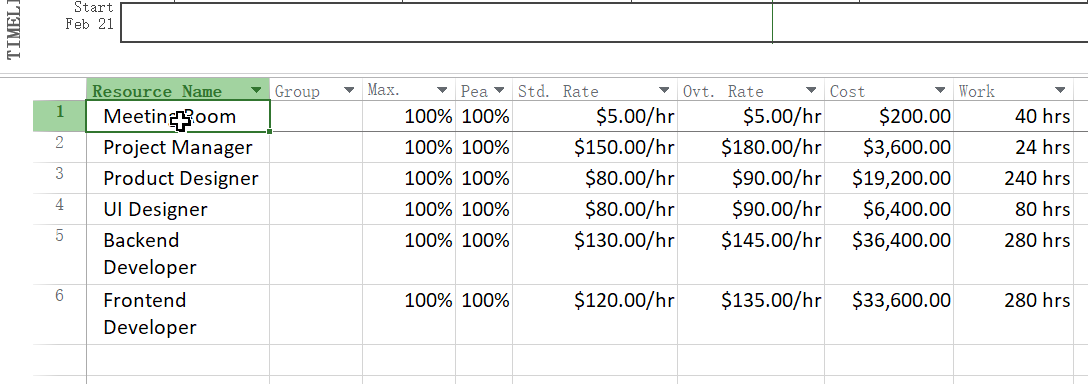
\includegraphics[width=1.0\textwidth]{./image/figure12}
    \caption{Resource Summary}
    \label{}
\end{figure}
\begin{figure}[H]
    \centering
    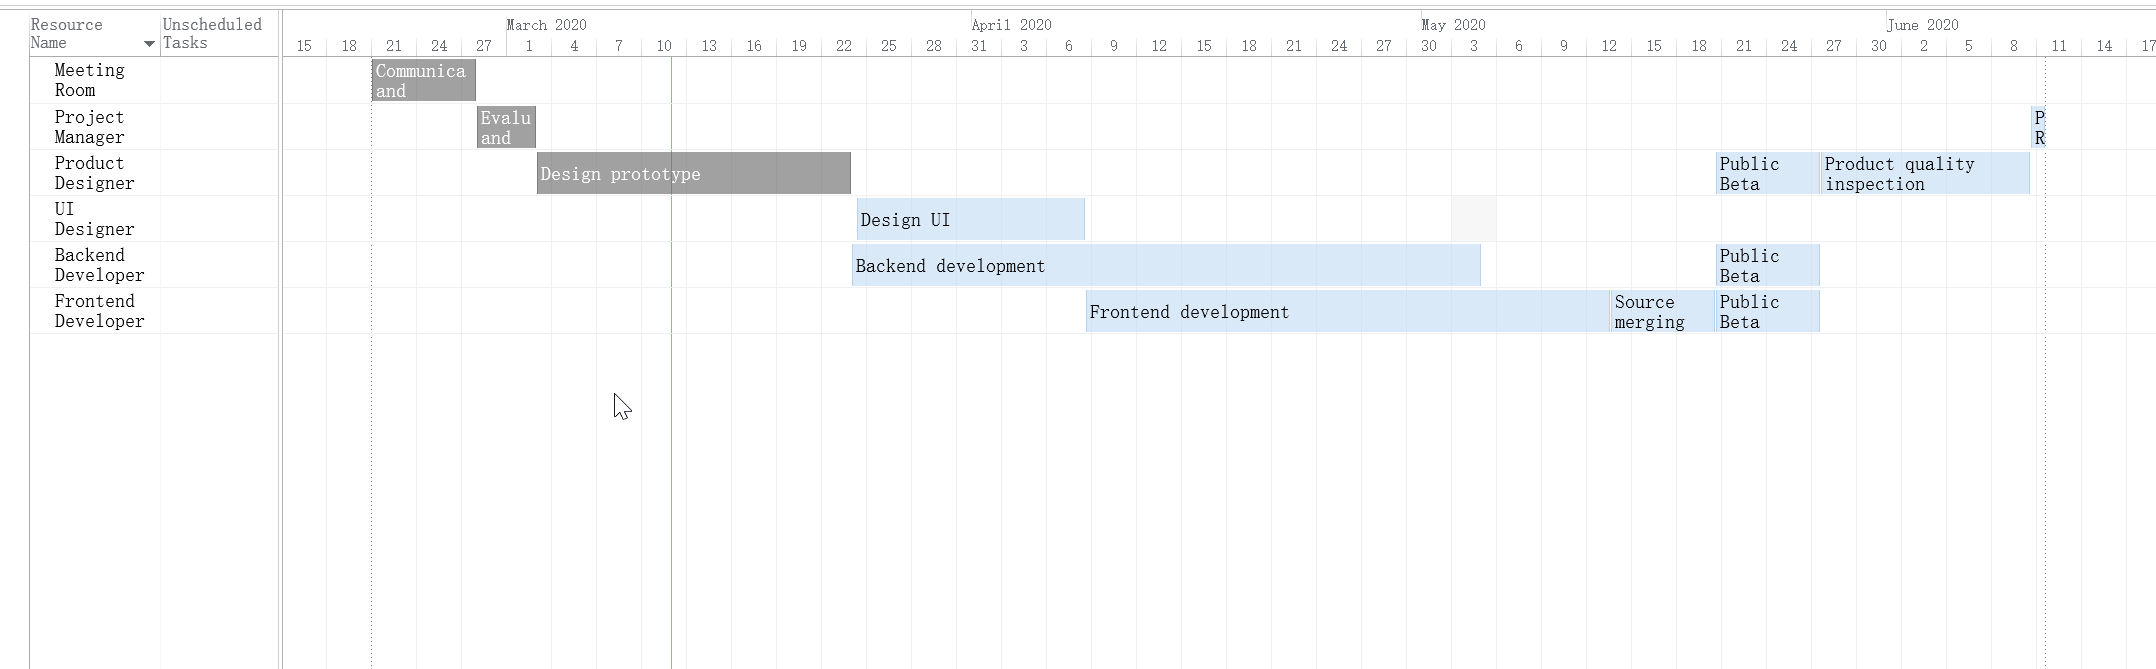
\includegraphics[width=1.0\textwidth]{./image/figure10}
    \caption{Gantt Chart1}
    \label{}
\end{figure}
\begin{figure}[H]
    \centering
    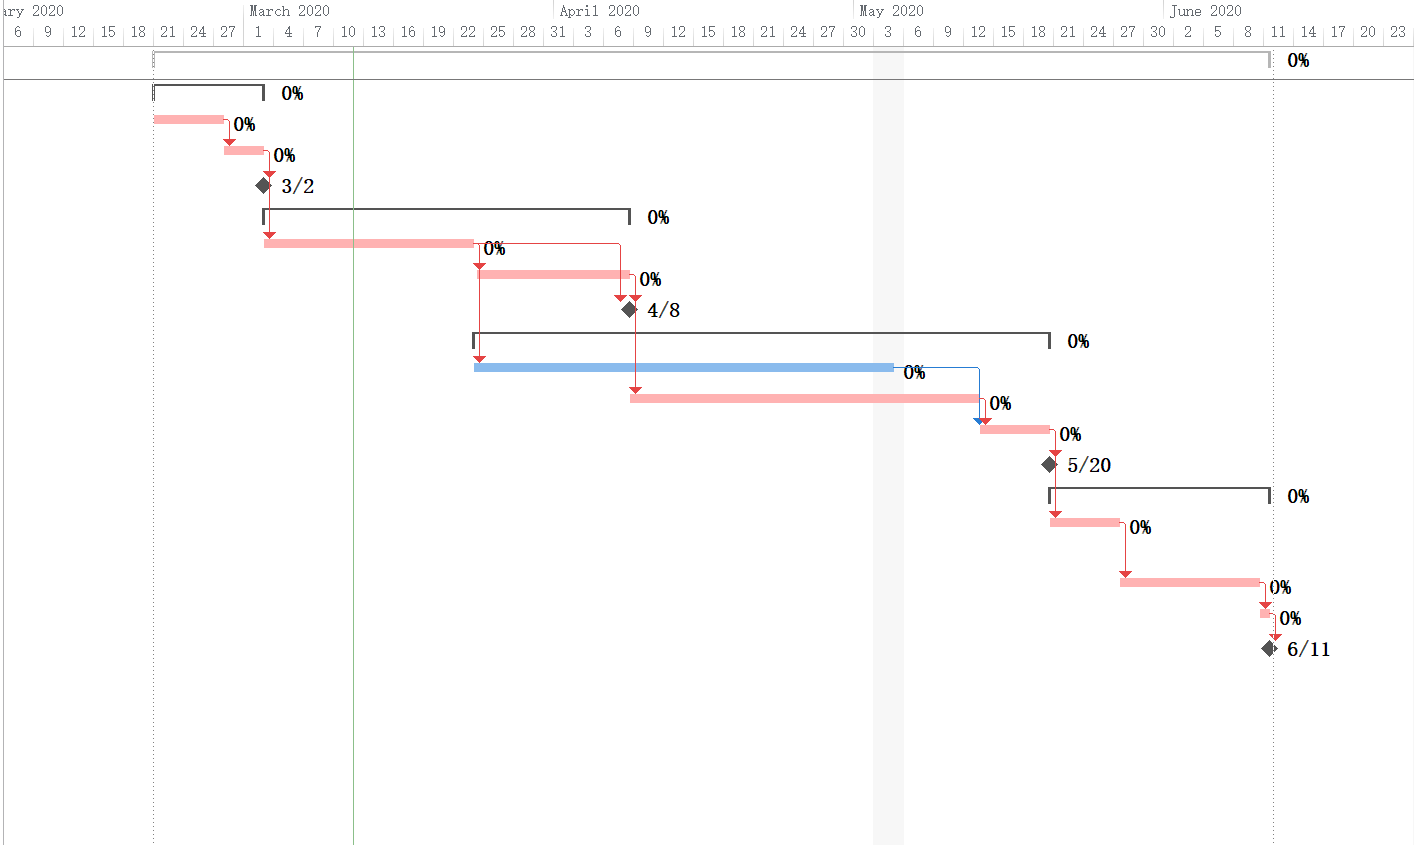
\includegraphics[width=1.0\textwidth]{./image/figure11}
    \caption{Gantt Chart2}
    \label{}
\end{figure}
\begin{figure}[H]
    \centering
    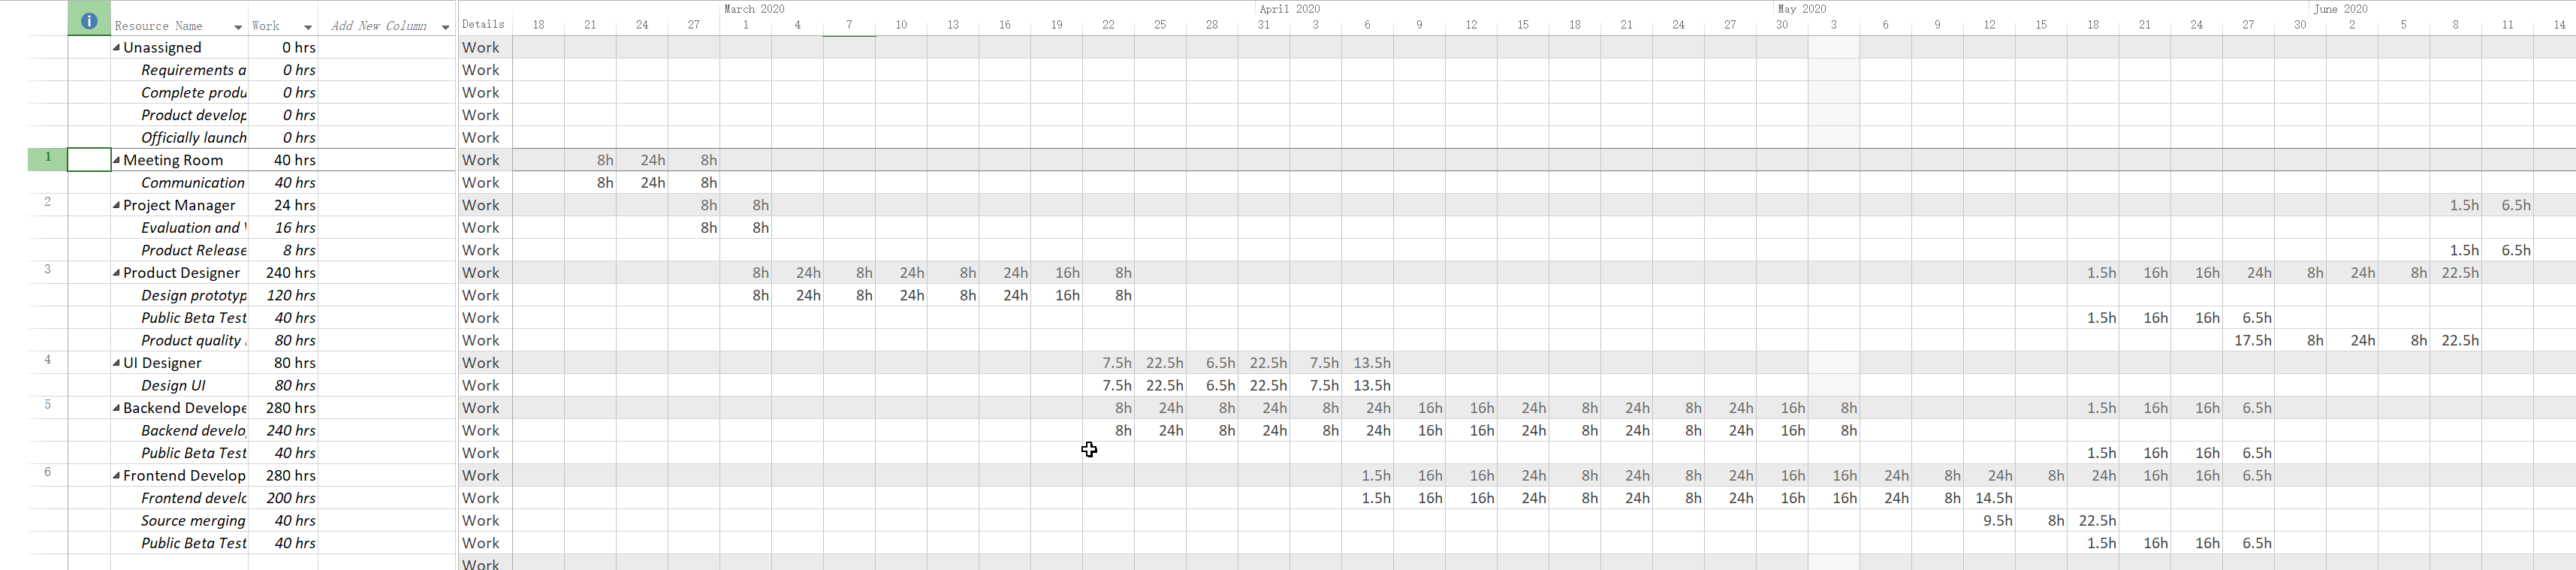
\includegraphics[width=1.0\textwidth]{./image/figure13}
    \caption{Resource usage plan}
    \label{}
\end{figure}


\end{document}